% !Mode:: "TeX:UTF-8"
% 20190804 commit
\documentclass[11pt,twoside]{ctexart}
\usepackage{geometry}
\usepackage{caption2,pifont,ulem}

\usepackage{tabto,yhmath}
\usepackage{amsmath,amssymb,amsthm}
\usepackage{fancyhdr}
\usepackage{tikz}
\usepackage{ifthen}

\usepackage{graphicx}
% \graphicspath{{figures/}}
\xeCJKsetcharclass{`①}{`⑩}{1}
\punctstyle{banjiao}%半角字符
\usepackage{enumitem}
% \setlist[enumerate,1]{itemsep=2pt,label=(\arabic*),labelsep=-0.3em,partopsep=0pt,parsep=\parskip,topsep=2pt,leftmargin=1.7em,align=left}
% \setlist[enumerate,2]{itemsep=2pt,label=\arabic*),labelsep=-1.0em,partopsep=0pt,parsep=\parskip,topsep=2pt,leftmargin=1.2em,align=left}
% \setitemize[1]{itemsep=0pt,partopsep=0pt,parsep=\parskip,topsep=0pt}
% \setdescription{itemsep=0pt,partopsep=0pt,parsep=\parskip,topsep=0pt}
\setlist[1]{labelindent=\parindent,leftmargin=2em,itemsep=0ex,partopsep=0pt,topsep=0pt,parsep=0.6ex}
\setlist[2]{labelindent=\parindent,leftmargin=2em,itemsep=0ex,partopsep=0pt,topsep=0pt,parsep=0.6ex}
% \usepackage{xeCJK}
\newcommand*{\fontdir}[1][fonts/]{\def\@fontdir{#1}}
\fontdir
% \renewcommand{\kaishu}{\relax}
\newCJKfontfamily\kai[
  Path={fonts/},
UprightFont=*,
]{kaiti_GB2312.ttf}

\newCJKfontfamily\biaosong[
  Path={fonts/},
UprightFont=*,
]{FZXBSJW.ttf}

\newCJKfontfamily\TimesNewRoman[
Path={fonts/},
UprightFont=*,
ItalicFont=*i,
BoldFont=*bd,
BoldItalicFont=*bi,
]{times.ttf}

\setmainfont[
Path={fonts/},
UprightFont=*,
ItalicFont=*i,
BoldFont=*bd,
BoldItalicFont=*bi,
]{times.ttf}

\newcommand*{\mifengxian}{%
\geometry{b4paper,twocolumn,landscape,hmargin={3.5cm,1cm},vmargin={1.5cm,1.5cm},footskip=0.75cm,headsep=0.25cm}
\pagestyle{fancy}
\renewcommand{\headrulewidth}{0pt}
\setlength{\columnseprule}{0.4pt}
\fancyfoot[CE,CO]{$-$\thepage$-$}
\fancyhead[CE,CO]{\mifengxianaaa}
}

\newcommand*{\mifengxianaaa}{%
\ifthenelse{\isodd{\value{page}}}%判断是否奇数页
{%B4正面密封线、座号
\begin{tikzpicture}[remember picture,overlay]
\path 	(current page.south east) coordinate (a0);
%定义右下角座号坐标
\draw 	(a0)[shift={(-2.5,0.83)}] node (a1) [draw=black,fill=gray!0,minimum height=1cm,minimum width=1cm]{\kaishu{}座号}
		(a1) node [right=0.5cm,draw=black,fill=gray!0,minimum height=1cm,minimum width=1cm]{};
\path 	(current page.west) coordinate (a0);
\draw 	(a0)[shift={(1.2,0)}] node (a1) [rotate=90,fill=gray!0,minimum height=1cm,minimum width=1cm]
		{\kaishu{}\zihao{4}
		学校\raisebox{-2pt}{\rule{35mm}{0.4pt}}%
		班级\raisebox{-2pt}{\rule{35mm}{0.4pt}}%
		姓名\raisebox{-2pt}{\rule{35mm}{0.4pt}}%
		考场\raisebox{-2pt}{\rule{35mm}{0.4pt}}%
		考号\raisebox{-2pt}{\rule{35mm}{0.4pt}}}
		(a1)[shift={(1.5,0)}] node [rotate=90,fill=gray!0,minimum height=1cm,minimum width=1cm]
		{\kaishu{}\zihao{4}...........................................%
		\raisebox{-0.6ex}{装}............................................%
		\raisebox{-0.6ex}{订}............................................%
		\raisebox{-0.6ex}{线}...........................................};
\end{tikzpicture}
}
{%B4反面装订线
\begin{tikzpicture}[remember picture,overlay]
\path 	(current page.east) coordinate (a0);
\draw 	(a0)[shift={(-2.7,0)}] node [rotate=-90,fill=gray!0,minimum height=1cm,minimum width=1cm]
		{\kaishu{}\zihao{4}...........................................%
		\raisebox{-0.6ex}{装}............................................%
		\raisebox{-0.6ex}{订}............................................%
		\raisebox{-0.6ex}{线}...........................................};
\end{tikzpicture}
}
}



%���Ų��Ͽ�,��������
\newcommand{\kh}{\unskip\nobreak\hfill\relpenalty=700\makebox[9.1mm][l]{(\qquad)}}

% ����ѡ��ʱ \xx{1}{2}
% ����ѡ��ʱ \xx{1}{2}{3}
% ...
% ���ѡ��ʱ \xx{1}{2}{3}{4}{5}

\usepackage{ifthen}
% \usepackage{enumitem}

\newlength{\testxxla}
\newlength{\testxxlb}
\newlength{\testxxlc}
\newlength{\testxxld}
\newlength{\testxxle}
\newlength{\lhalf}
\newlength{\ltrisect}
\newlength{\lquarter}
\newlength{\lfifth}
\newlength{\lmax}

%-----------------------------------------------------------------------------%
% �ޱ�ǩ����ѡ������ʽ��һ�ж�ѡ��
%-----------------------------------------------------------------------------%
\newcommand{\testtwo}[2]
{%\par\noindent%
    \settowidth{\testxxla}{A.~#1~~~}
    \settowidth{\testxxlb}{B.~#2~~~}
	 \ifthenelse{\lengthtest{\testxxla>\testxxlb}}{\setlength{\lmax}{\testxxla}}{\setlength{\lmax}{\testxxlb}}
	\setlength{\lhalf}{0.47\linewidth}%
	\ifthenelse{\lengthtest{\lmax>\lhalf}}
    {
        \begin{enumerate}[label=\Alph*.,parsep=0ex,itemsep=0ex,leftmargin=6mm, topsep=0ex]
            \item #1
            \item #2
        \end{enumerate}
    }
	{
	\makebox[\lhalf][l]{A.~#1~~~}%
	\makebox[\lhalf][l]{B.~#2~~~}%
	}
}
%-----------------------------------------------------------------------------%
% ��ѡ�����ѡ��ij����Զ��ж������ʽ��һ��һѡ�һ�ж�ѡ�һ����ѡ��
%-----------------------------------------------------------------------------%
\newcommand{\testxxfour}[4]
{
    % \par
    \settowidth{\testxxla}{A.~#1~~~}
    \settowidth{\testxxlb}{B.~#2~~~}
    \settowidth{\testxxlc}{C.~#3~~~}
    \settowidth{\testxxld}{D.~#4~~~}
    \ifthenelse{\lengthtest{\testxxla>\testxxlb}}{\setlength{\lmax}{\testxxla}}{\setlength{\lmax}{\testxxlb}}
    \ifthenelse{\lengthtest{\testxxlc>\lmax}}{\setlength{\lmax}{\testxxlc}}{}
    \ifthenelse{\lengthtest{\testxxld>\lmax}}{\setlength{\lmax}{\testxxld}}{}
    \setlength{\lhalf}{0.47\linewidth}
    \setlength{\lquarter}{0.23\linewidth}
    \ifthenelse{\lengthtest{\lmax>\lhalf}}
    {%\vspace*{-4mm}
        \begin{enumerate}[label=\Alph*.,parsep=0ex,itemsep=0ex,leftmargin=6mm, topsep=0ex]
            \item #1
            \item #2
            \item #3
            \item #4
        \end{enumerate}
    }
    {
        \ifthenelse{\lengthtest{\lmax>\lquarter}}
        {
            \noindent%
            \makebox[\lhalf][l]{A.~#1~~~}%
            \makebox[\lhalf][l]{B.~#2~~~}%
            \par\noindent%
            \makebox[\lhalf][l]{C.~#3~~~}%
            \makebox[\lhalf][l]{D.~#4~~~}%
        }%
        {
            \noindent%
            \makebox[\lquarter][l]{A.~#1~~~}%
            \makebox[\lquarter][l]{B.~#2~~~}%
            \makebox[\lquarter][l]{C.~#3~~~}%
            \makebox[\lquarter][l]{D.~#4~~~}%
        }
    }
}
%-----------------------------------------------------------------------------%
% ��ѡ�����ѡ��ij����Զ��ж������ʽ��һ��һѡ�һ�ж�ѡ�һ����ѡ��
%-----------------------------------------------------------------------------%
\newcommand{\testxxfive}[5]
{
    \par
    \settowidth{\testxxla}{A.~#1~~~}
    \settowidth{\testxxlb}{B.~#2~~~}
    \settowidth{\testxxlc}{C.~#3~~~}
    \settowidth{\testxxld}{D.~#4~~~}
    \settowidth{\testxxle}{E.~#5~~~}
    \ifthenelse{\lengthtest{\testxxla>\testxxlb}}{\setlength{\lmax}{\testxxla}}{\setlength{\lmax}{\testxxlb}}
    \ifthenelse{\lengthtest{\testxxlc>\lmax}}{\setlength{\lmax}{\testxxlc}}{}
    \ifthenelse{\lengthtest{\testxxld>\lmax}}{\setlength{\lmax}{\testxxld}}{}
    \ifthenelse{\lengthtest{\testxxle>\lmax}}{\setlength{\lmax}{\testxxle}}{}
    \setlength{\lhalf}{0.47\linewidth}
    \setlength{\ltrisect}{0.31\linewidth}
    \setlength{\lquarter}{0.23\linewidth}
    \setlength{\lfifth}{0.18\linewidth}
    \ifthenelse{\lengthtest{\lmax>\lhalf}}
    {
        \begin{enumerate}[label=\Alph*.,parsep=0ex,itemsep=0ex,leftmargin=6mm, topsep=0ex]
            \item #1
            \item #2
            \item #3
            \item #4
            \item #5
        \end{enumerate}
    }
    {
        \ifthenelse{\lengthtest{\lmax>\ltrisect}}
        {\kh
            \noindent%
            \makebox[\lhalf][l]{A.~#1~~~}%
            \makebox[\lhalf][l]{B.~#2~~~}%
            \par\noindent%
            \makebox[\lhalf][l]{C.~#3~~~}%
            \makebox[\lhalf][l]{D.~#4~~~}%
            \par\noindent%
            \makebox[\lhalf][l]{E.~#5~~~}%
            \makebox[\lhalf][l]{}%
        }
        {
            \ifthenelse{\lengthtest{\lmax>\lquarter}}
            {\kh
                \noindent%
                \makebox[\ltrisect][l]{A.~#1~~~}%
                \makebox[\ltrisect][l]{B.~#2~~~}%
                \makebox[\ltrisect][l]{C.~#3~~~}%
                \par\noindent%
                \makebox[\ltrisect][l]{D.~#4~~~}%
                \makebox[\ltrisect][l]{E.~#5~~~}%
                \makebox[\ltrisect][l]{}%
            }
            {
                \ifthenelse{\lengthtest{\lmax>\lfifth}}
                {
                    \noindent%
                    \makebox[\lquarter][l]{A.~#1~~~}%
                    \makebox[\lquarter][l]{B.~#2~~~}%
                    \makebox[\lquarter][l]{C.~#3~~~}%
                    \makebox[\lquarter][l]{D.~#4~~~}%
                    \par\noindent%
                    \makebox[\lquarter][l]{E.~#5~~~}%
                    \makebox[\lquarter][l]{}%
                    \makebox[\lquarter][l]{}%
                    \makebox[\lquarter][l]{}%
                }
                {
                    \noindent%
                    \makebox[\lfifth][l]{A.~#1~~~}%
                    \makebox[\lfifth][l]{B.~#2~~~}%
                    \makebox[\lfifth][l]{C.~#3~~~}%
                    \makebox[\lfifth][l]{D.~#4~~~}%
                    \makebox[\lfifth][l]{E.~#5~~~}%
                }
            }
        }
    }
}
%-----------------------------------------------------------------------------%
% ��ѡ�����ѡ��ij����Զ��ж������ʽ��һ��һѡ�һ�ж�ѡ�һ����ѡ��
%-----------------------------------------------------------------------------%
\newcommand{\testxxthree}[3]
{
    \par
    \settowidth{\testxxla}{A.~#1~~~}
    \settowidth{\testxxlb}{B.~#2~~~}
    \settowidth{\testxxlc}{C.~#3~~~}
    \ifthenelse{\lengthtest{\testxxla>\testxxlb}}{\setlength{\lmax}{\testxxla}}{\setlength{\lmax}{\testxxlb}}
    \ifthenelse{\lengthtest{\testxxlc>\lmax}}{\setlength{\lmax}{\testxxlc}}{}
    \setlength{\lhalf}{0.47\linewidth}
    \setlength{\ltrisect}{0.31\linewidth}
    \ifthenelse{\lengthtest{\lmax>\lhalf}}
    {
        \begin{enumerate}[label=\Alph*.,parsep=0ex,itemsep=0ex,leftmargin=6mm, topsep=0ex]
            \item #1
            \item #2
            \item #3
        \end{enumerate}
    }
    {
        \ifthenelse{\lengthtest{\lmax>\ltrisect}}
        {
            \noindent%
            \makebox[\lhalf][l]{A.~#1~~~}%
            \makebox[\lhalf][l]{B.~#2~~~}%
            \par\noindent%
            \makebox[\lhalf][l]{C.~#3~~~}%
        }%
        {
            \noindent%
            \makebox[\ltrisect][l]{A.~#1~~~}%
            \makebox[\ltrisect][l]{B.~#2~~~}%
            \makebox[\ltrisect][l]{C.~#3~~~}%
        }
    }
}


\makeatletter
\newcommand{\xx@i}[2]{\testtwo{#1}{#2}}
\newcommand{\xx@ii}[3]{\testxxthree{#1}{#2}{#3}}
\newcommand{\xx@iii}[4]{\testxxfour{#1}{#2}{#3}{#4}}
\newcommand{\xx@iv}[5]{\testxxfive{#1}{#2}{#3}{#4}{#5}}
\newcommand{\xx@iii@helper}[4]{%
	\@ifnextchar\bgroup
	{\xx@iv{#1}{#2}{#3}{#4}}{\xx@iii{#1}{#2}{#3}{#4}}}
\newcommand{\xx@ii@helper}[3]{%
	\@ifnextchar\bgroup
	{\xx@iii@helper{#1}{#2}{#3}}{\xx@ii{#1}{#2}{#3}}}
\newcommand{\xx}[2]{%
	\hfill\kh\par\@ifnextchar\bgroup
	{\xx@ii@helper{#1}{#2}}{\xx@i{#1}{#2}}}
\makeatother


\graphicspath{{figures/}{figures9/}}
\mifengxian

update github
\begin{document}
%
%	试卷标题
%
\begin{center}\biaosong
\zihao{3}{$2018$---$2019$学年下学期九年级第一次阶段性考试~~~数学试卷}\\
{\kai\zihao{5}{时间:100分钟~~~~~满分:120分}}
\end{center}
%
%	试卷正面
%
\begin{enumerate}
\item[\!\!\!\!\kai{}一]{\makebox[0mm][r]{\!\!\!、}\kai{}选择题(每小题3分,共30分)}%-------------------------------------选择题

% 1
\item $-0.2$的相反数是
\xx
{$0.2$}
{$\pm0.2$}
{$-0.2$}
{$2$}

% 2
\item 
下列四个图形中,既是轴对称图形又是中心对称图形的个数为
\xx{1个}{2个}{3个}{4个}

\begin{center}
\hskip-2em
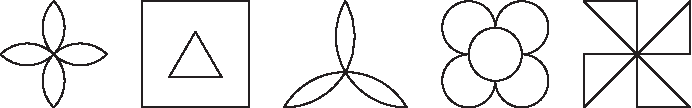
\includegraphics{fig1.pdf}
\end{center}

% \item 用平面去截一个几何体,如截面为长方形,则几何体不可能是
% \xx{圆柱}{圆锥}{长方体}{正方体}
% 3
\item 一个正方体切去一个三棱锥后所得几何体的俯视图是\hfill\kh

\begin{center}
\hskip-2em
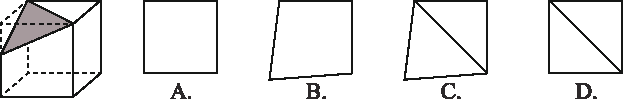
\includegraphics{fig2.pdf}
\end{center}


% 4
\item 方程$\dfrac{1}{x-2}-1=\dfrac{3}{2-x}$的解为
\xx
{$x=4$}
{$x=-3$}
{$x=6$}
{此方程无解}

% 5
\item 下列调查中,最适宜采用全面调查方式的是
\xx
{对三门峡全市初中学生每天学习所用时间的调查}
{对全国中学生心理健康现状的调查}
{对某班学生进行6月5日是``世界环境日''知晓情况的调查}
{对三门峡全市初中学生视力情况的调查\tabto{.7\columnwidth}\vbox{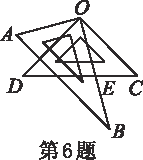
\includegraphics{fig03.pdf}}}



% 6
\item 如图,将一副三角板叠放在一起,使直角的顶点重合于点$O$,$AB//OC$,$DC$与$OB$交于点$E$,则$\angle DEO$的度数为
\xx
{$85^{\circ}$}
{$70^{\circ}$}
{$75^{\circ}$}
{$60^{\circ}$}

% 7
\item 关于$x$的一元二次方程$(a-3)x^2-\sqrt{17}x+1=0$有实数根,则实数$a$满足
\xx
{$a<\frac{29}{4}$}
{$a\geqslant \frac{29}{4}$}
{$a\leqslant \frac{29}{4}$且$a\ne3$}
{$a\geqslant \frac{29}{4}$且$a\ne3$}

% 8
\item 若$A(-4,y_1)$,$B(-3,y_2)$,$C(1,y_3)$为二次函数$y=x^2-4x+m$的图象上的三点,则$y_1$,$y_2$,$y_3$的大小关系是
\xx
{$y_1<y_2<y_3$}
{$y_3<y_2<y_1$}
{$y_3<y_1<y_2$}
{$y_1<y_3<y_2$}



% 9
\item 
\begin{minipage}[t]{0.35\textwidth}
如图,在$\triangle OAB$中,$OA=OB$,$\angle AOB=15^{\circ }$,在$\triangle OCD$中,$OC=OD$,$\angle COD=45^{\circ }$,且点$C$在边$OA$上,连接$CB$,将线段$OB$绕点$O$逆时针旋转一定角度得到线段$OE$,使得$DE=CB$,则$\angle BOE$的度数为
\xx
{15$^{\circ}$}
{15$^{\circ}$或45$^{\circ}$}
{45$^{\circ}$}
{45$^{\circ}$或60$^{\circ}$}
\hspace*{1.03\textwidth}\vbox{\makebox[0mm][l]{\raisebox{3.5ex}[0cm][0cm]{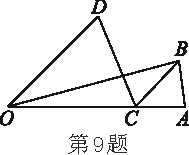
\includegraphics{fig04.pdf}}}}\null
\end{minipage}


% 10
\item 
如图,正方形$ABCD$的边长为4,点$P$,$Q$分别是$CD$,$AD$的中点,动点$E$从点$A$向点$B$运动,到点$B$时停止运动;同时,动点$F$从点$P$出发,沿$P\to D\to Q$运动,点$E$,$F$的运动速度相同.设点$E$的运动路程为$x$,$\triangle AEF$的面积为$y$,能大致刻画$y$与$x$的函数关系的图象是\hfill\kh
\begin{center}
\hskip-1.2em
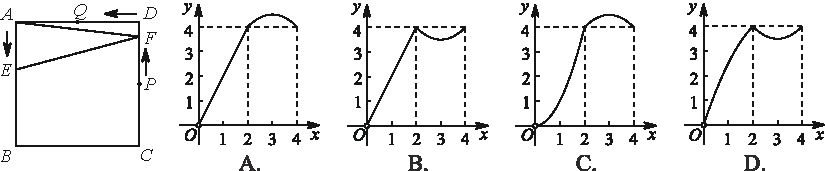
\includegraphics{fig05.pdf}
\end{center}




\item[\!\!\!\!\kai{}二]{\makebox[0mm][r]{\!\!\!、}\kai{}填空题(每空3分,共15分)}%--------------------------------------填空题
% 11 
\item 
计算:$\sqrt 4  + ( - 2)^0= \underline{\hspace*{3cm}}$.
% 12
\item
关于$x$的一元二次方程$x^2-6x+b=0$有两个不相等的实数根,则实数$b$的取值范围是\underline{\hspace*{2cm}}.
% 13
\item 
一名射击运动员连续打靶8次,命中的环数如图所示,这组数据的众数是\underline{\hspace*{2cm}}.
\begin{center}
\hskip-1.2em
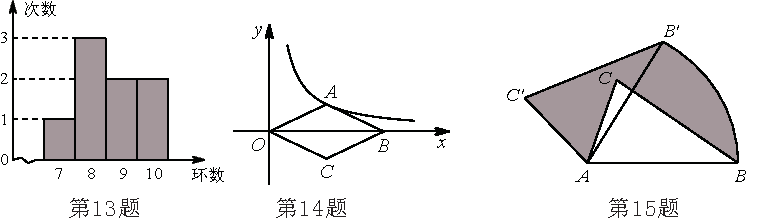
\includegraphics[scale=1]{fig06a.pdf}
\end{center}
% 14
\item
如图,在平面直角坐标系中,点$O$为原点,菱形$OABC$的对角线$OB$在$x$轴上,顶点$A$在反比例函数$y=\dfrac{1}{x}$的图象上,则菱形的面积为\underline{\hspace*{2cm}}.

% 15
\item 
如图,在等腰$\triangle ABC$中,$\angle CAB>60^{\circ }$,$AB=BC=2$,在同一平面内,将$\triangle ABC$绕点$A$逆时针旋转60$^{\circ }$得到$\triangle AB'C'$,$\wideparen{BB'}$为$B$的运动轨迹,则图中阴影部分的面积为\underline{\hspace*{2cm}}.

\clearpage
\setcounter{enumi}{15}


\item[\!\!\!\!\kai{}三]{\makebox[0mm][r]{\!\!\!、}\kai{}解答题(共75分)}%-----------------------------------------------解答题
\item (8分)先化简,再求值:$\dfrac{2}{a-1}-\dfrac{a+1}{a^2-2a+1}\div \dfrac{a+1}{a-1}$,其中$a=\sqrt 2 +1$.
\vfill
\vfill
\item 
(9分)某小学开展寒假争星活动,学生可以从“自理星”、“读书星”、“健康星”、“孝敬星”等中选一个项目参加争星竞选.根据该校一年级某班学生的“争星”报名情况,绘制成了如下两幅不完整的统计图,请根据图中信息回答下列问题:
\begin{center}
\hskip-1.2em
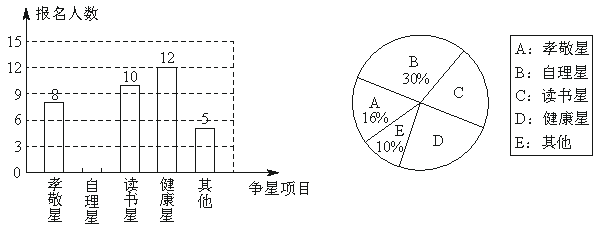
\includegraphics[scale=1.2]{fig07.pdf}
\end{center}

(1)参加调查的学生共有\underline{\hspace*{2cm}}人;\\
(2)将条形统计图补充完整;\\
(3)请计算扇形统计图中“读书星”对应的扇形圆心角度数;\\
(4)根据调查结果,试估计该小学全校3600名学生中争当“健康星”的学生人数.

\vfill\null\newpage

\item
(9分)如图,在$\triangle ABC$中,$AB=10\sqrt 2 $,$\angle BAC=60^{\circ }$,$\angle B=45^{\circ }$,点$D$是$BC$边上一动点,连接$AD$,以$AD$为直径作$\odot O$交边$AB$,$AC$于点$E$,$F$,连接$OE$,$OF$,$DE$,$DF$,$EF$.
\\
(1)求$\dfrac{EF}{OE}$的值;\\
(2)填空:①当$AD$平分$\angle BAC$时,四边形$OEDF$的形状是\underline{\hspace*{2cm}};
\\
②点$D$在运动过程中,线段$EF$的最小值为\underline{\hspace*{2cm}}.

% \tabto{0.3\textwidth}
\hfill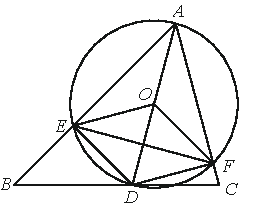
\includegraphics[scale=1]{fig08.pdf}\quad
\vfill

\item
(9分)一轮船在$P$处测得灯塔$A$在正北方向,灯塔$B$在南偏东30$^{\circ }$方向,轮船向正东航行了900~m,到达$Q$处,测得$A$位于北偏西60$^{\circ }$方向,$B$位于南偏西30$^{\circ }$方向.
\\
(1)线段$BQ$与$PQ$是否相等?请说明理由;\\
(2)求$A$,$B$间的距离(结果保留根号).

\hfill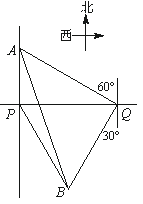
\includegraphics[scale=1.4]{fig09.pdf}\quad
\vfill
\vfill
\null
\newpage

\item
(9分)如图,在同一直角坐标系中,直线$y=x+4$与$y=-3x-3$相交于$A$点,分别与$x$轴交于$B$,$C$两点.
\\
(1)求$\triangle ABC$的面积;\\
(2)$P$,$Q$分别为直线$y=x+4$与$y=-3x-3$上的点,且$P$,$Q$关于原点对称,求$P$点的坐标.

\hfill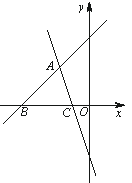
\includegraphics[scale=1.5]{fig10.pdf}\quad


\item
(10分)某商城销售A,B两种型号高档变速自行车.A型自行车售价为2100元/辆,B型自行车售价为1 750元/辆,每辆A型自行车的进价比每辆B型自行车的进价多400元,商城用80 000元购进A型自行车的数量与用64000元购进B型自行车的数量相等.\\
(1)求每辆A,B两种自行车的进价分别是多少?\\
(2)现在商城准备一次购进这两种自行车共100辆.设购进A型自行车$m$辆,这100辆自行车的销售总利润为$y$元.要求购进B型自行车数量不超过A型自行车数量的2倍,总利润不低于13 000元,求获利最大的方案以及最大利润.

\vfill
\newpage

\item
(10分)在$\triangle ABC$中,$\angle ACB$是锐角,点$D$在射线$BC$上运动,连接$AD$,将线段$AD$绕点$A$逆时针旋转90$^{\circ }$,得到$AE$,连接$EC$.\\
(1)操作发现:若$AB=AC$,$\angle BAC=90^{\circ }$,当$D$在线段$BC$上时(不与点$B$重合),如图1所示,请你直接写出线段$CE$和$BD$的位置关系是\underline{\hspace*{2cm}},数量关系是\underline{\hspace*{2cm}};\\
(2)猜想论证:在(1)的条件下,当$D$在线段$BC$的延长线上时,如图2所示,请你判断(1)中结论是否成立,并证明你的判断;\\
(3)拓展延伸:如图3,若$AB\neq AC$,$\angle BAC\neq90^{\circ }$,点$D$在线段$BC$上运动,试探究:当锐角$\angle ACB$等于\underline{\hspace*{2cm}}度时,线段$CE$和$BD$之间的位置关系仍成立(点$C$,$E$重合除外)?此时若作$DF\bot AD$交线段$CE$于点$F$,且当$AC=3\sqrt2$时,请直接写出线段$CF$的长的最大值是\underline{\hspace*{2cm}}.

\hfill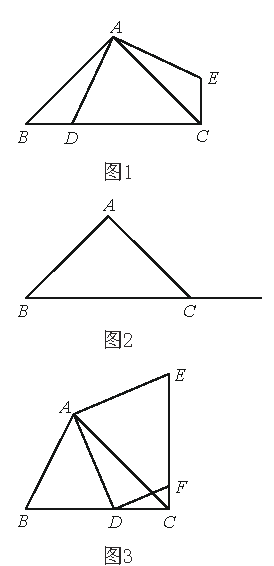
\includegraphics[scale=1.05]{fig11.pdf}\quad

\vfill
\newpage
\item 
(11分)如图,已知抛物线$y=x^2+bx+c$与$x$轴交于$A$,$B$两点,与$y$轴交于点$C$,直线$y=2x-8$经过$B$,$C$两点.\\
(1)求抛物线的表达式.\\
(2)点$D$是线段$BC$上一动点,过点$D$作$x$轴的垂线交抛物线于点$M$,求线段$DM$长度的最大值.\\
(3)线段$DE=\sqrt5$,当线段$DE$(点$E$在点$D$的下方)在线段$BC$上滑动时,是否存在以$D$,$M$,$E$为顶点的三角形和$\triangle BOC$相似?若存在,直接写出所有符合条件的点$M$的横坐标;若不存在,请说明理由.

\hfill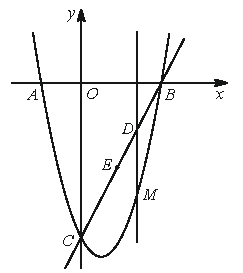
\includegraphics[scale=1.05]{fig12.pdf}\quad
\iffalse
\fi
\end{enumerate}
\end{document}
